\chapter{Démonstration des outils Tufte}

\section{Notes de marge}
Voici une phrase utilisant une \verb|\sidenote|\sidenote{Ceci est une note de marge numérotée.} pour donner un détail. Si vous voulez juste une remarque sans numéro, utilisez \verb|\marginnote|\marginnote{Attention : ceci est une note libre sans appel dans le texte.} dans la marge.

\section{Éléments visuels dans la marge}
Vous pouvez intégrer des figures étroites avec \verb|\begin{marginfigure}|.
\begin{marginfigure}
	\centering
	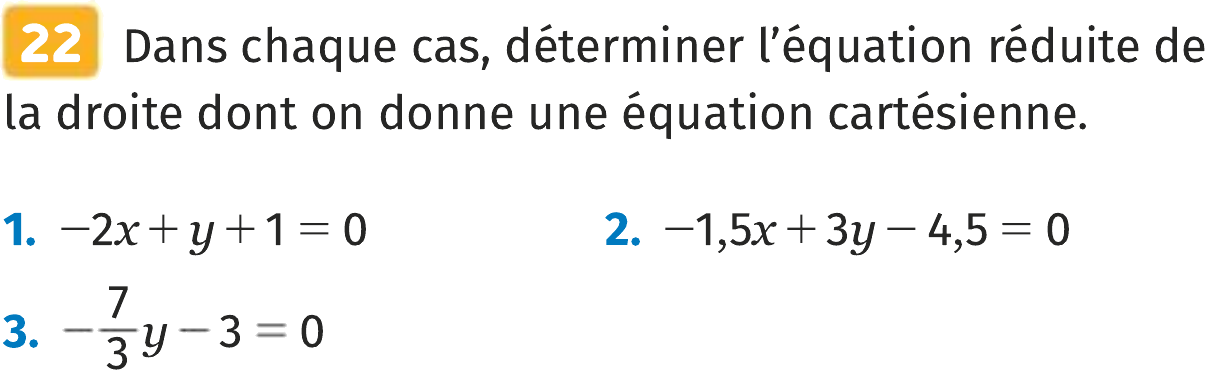
\includegraphics[width=\linewidth]{img/22.png}
	\caption{Légende de la figure en marge.}
\end{marginfigure}

Ou des tableaux compacts avec \verb|\begin{margintable}|.
\begin{margintable}
	\centering
	\begin{tabular}{ll}
		Objet & Valeur \\
		\hline
		$x$   & 10     \\
		$y$   & 20     \\
	\end{tabular}
	\caption{Tableau de données en marge.}
\end{margintable}

\section{Typographie et Styles}
\newthought{La mise en page Tufte}\sidenote{Avec \texttt{\textbackslash newthought}} repose sur une typographie soignée. Ici, l'utilisation de la commande \texttt{\textbackslash newthought} permet d'introduire un nouveau sujet de manière élégante, avec un léger retrait et des petites capitales.

\ms

Le style Tufte utilise des effets typographiques pour le confort visuel :
\begin{itemize}
	\item Texte en \allcaps{MAJUSCULES ESPACÉES} pour les titres ou acronymes \bi\item $\rarr$ \verb|\allcaps{}|\ei
	\item Texte en \smallcaps{petites capitales} pour un rendu classique \bi\item $\rarr$ \verb|\smallcaps{}|\ei
\end{itemize}

\section{Pleine largeur}
Pour un élément massif, utilisez l'environnement pleine largeur :
\begin{fullwidth}
	Voici un bloc de texte qui ignore totalement la marge latérale pour occuper toute la largeur disponible de la page. C'est idéal pour des équations complexes :
	\[ \int_{-\infty}^{+\infty} e^{-x^2} dx = \sqrt{\pi} \]
\end{fullwidth}

C'est l'environnement \verb|\begin{fullwidth}|.

\newpage

\cimg{10cm}{img/100.png}

\lipsum[1] % Texte de remplissage

\section{ma section}

% \begin{defin}
% 	Soit $f$ une fonction définie sur un intervalle $I \subset \mathbb{R}$. Pour tout $x \in I$, le réel $f(x)$ est appelé l'image de $x$ par la fonction $f$.
% \end{defin}

\begin{marginfigure}
	\centering
	
\includegraphics[width=\linewidth]{img/barbaraalane-fractal-1784703_1920.jpg}
	\caption{Exercice du chapitreeee}
	\label{fig:ma_figure_marge}
\end{marginfigure}

% \begin{prop}
% 	Soit $f$ une fonction affine définie sur $\mathbb{R}$ par $f(x) = ax + b$.
% 	Si $a > 0$, alors $f$ est strictement croissante sur $\mathbb{R}$.
% \end{prop}
%
% \begin{theo}
% 	Pour tous réels $a$ et $b$, on a l'identité remarquable suivante :
% 	\[ (a+b)^2 = a^2 + 2ab + b^2 \]
% \end{theo}

\subsection{et une subsection}

% \begin{methode}
% 	Pour résoudre l'équation\sidenote{Ouh c'est chaud !\par\noindent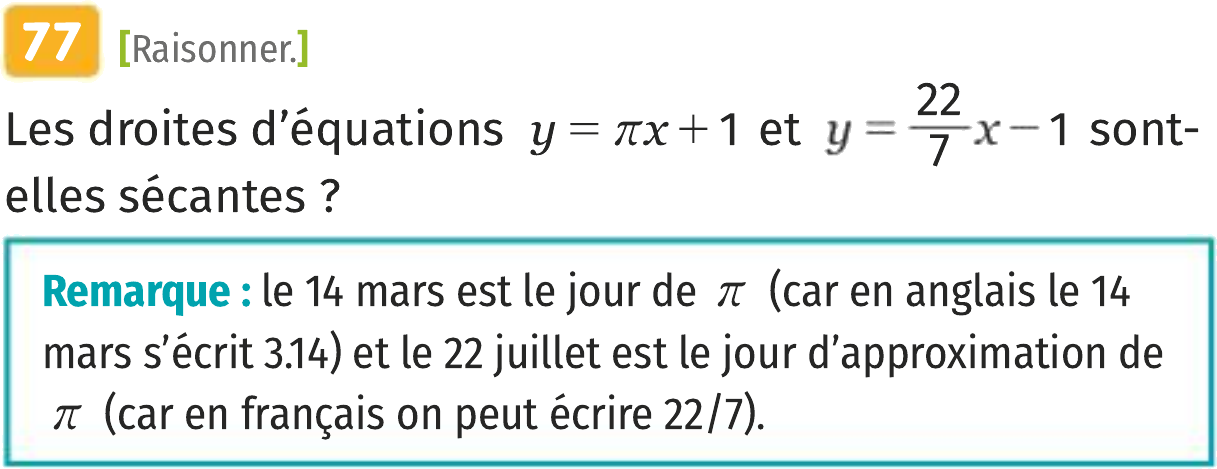
\includegraphics[width=\linewidth]{img/77.png}} $x^2 - 9 = 0$ :
% 	\begin{enumerate}
% 		\item On reconnaît une différence de deux carrés : $x^2 - 3^2 = 0$.
% 		\item On factorise : $(x-3)(x+3) = 0$.
% 		\item On utilise la propriété du produit nul.
% 	\end{enumerate}
% \end{methode}
%
% \begin{ex}[Super exemple des familles]
% 	Développons l'\ul{expression} $A = (2x+1)(x-4)$ :
% 	\[ A = 2x^2 - 8x + x - 4 = 2x^2 - 7x - 4 \]
% \end{ex}
%
% \begin{attention}
% 	Il ne faut pas confondre $f(x+h)$ et $f(x) + h$. En général, $f(x+h) \neq f(x) + h$.
% \end{attention}
%
% \begin{demo}
% 	Montrons que $(a+b)^2 = a^2 + 2ab + b^2$ :
%
% 	$$
% 		\begin{array}{rcl}
% 			(a+b)^2 & = & (a+b)(a+b)          \\
% 			        & = & a(a+b) + b(a+b)     \\
% 			        & = & a^2 + ab + ba + b^2 \\
% 			        & = & a^2 + 2ab + b^2
% 		\end{array}
% 	$$
%
% \end{demo}

\section{plop plop}

En pleine largeur \verb|\begin{fullwidth}| :

\begin{fullwidth}
	\begin{lstlisting}[caption={Simulation d'une variable aléatoire et calcul de la moyenne empirique}]
import numpy as np

def simuler_loi(n, p=0.5):
	"""
	Simule n variables de Bernoulli de parametre p.
	"""
	# Génération de n échantillons aléatoires
	echantillon = np.random.binomial(1, p, n)

	# Calcul de la moyenne empirique
	moyenne = np.mean(echantillon)

	return moyenne

# Exécution et affichage des résultats
if __name__ == "__main__":
	n_essais = 1000
	resultat = simuler_loi(n_essais)
	print(f"Moyenne empirique pour {n_essais} essais : {resultat}")
			\end{lstlisting}
\end{fullwidth}

et en normal :

\begin{lstlisting}
def calculer_moyenne(liste):
    # Calcul de la somme
    somme = sum(liste)
    return somme / len(liste)

# Test de la fonction
resultat = calculer_moyenne([10, 15, 20])
print(resultat)
\end{lstlisting}

\subsection{asdasd sdsd}

\lipsum[2]
